\documentclass{amsart}
\synctex=1

%=================================================================
% 
\newcount\DraftStatus  % 0 suppresses notes to selves in text
\DraftStatus=1   % TODO: set to 0 for final version
%=================================================================

%=================================================================
\usepackage{comment}
%=================================================================
%
\includecomment{JournalOnly}  
\includecomment{ConferenceOnly}  
\includecomment{TulipStyle}
%
%=================================================================
%=================================================================
% gitlatexdiff
%
%  https://gitlab.com/git-latexdiff/git-latexdiff
%=================================================================
%  git latexdiff HEAD  HEAD~5 --main templatex.tex
%  git latexdiff HEAD~1  --main templatex.tex
%  View pdf to see difference
%
%=================================================================
%
% Todo Notes for marginal comments
% 
%\newcount\DraftStatus  % 0 suppresses notes to selves in text
%\DraftStatus=1   % TODO: set to 0 for final version
\ifnum\DraftStatus=1
	\usepackage[draft,colorinlistoftodos,color=orange!30]{todonotes}
\else
	\usepackage[disable,colorinlistoftodos,color=blue!30]{todonotes}
\fi 
%\usepackage[disable]{todonotes} % notes not showed
%\usepackage[draft]{todonotes}   % notes showed
%
\makeatletter
 \providecommand\@dotsep{5}
 \def\listtodoname{List of Todos}
 \def\listoftodos{\@starttoc{tdo}\listtodoname}
 \makeatother
%
%=================================================================
%
\usepackage{color}
\newcommand{\draftnote}[3]{ 
	\todo[author=#2,color=#1!30,size=\footnotesize]{\textsf{#3}}	}
% TODO: add yourself here:
%
\newcommand{\gangli}[1]{\draftnote{blue}{GLi:}{#1}}
\newcommand{\qwu}[1]{\draftnote{red}{QWu:}{#1}}
\newcommand{\gliMarker}
	{\todo[author=GLi,size=\tiny,inline,color=blue!40]
	{Gang Li has worked up to here.}}
\newcommand{\qwuMarker}
	{\todo[author=QWu,size=\tiny,inline,color=red!40]
	{Qiong Wu has worked up to here.}}
%=================================================================

%=================================================================
%
% general packages
%  https://en.wikibooks.org/wiki/Category:Book:LaTeX
%  https://en.wikibooks.org/wiki/LaTeX/Package_Reference
%
%=================================================================
\usepackage{graphicx}
\usepackage{algorithm}
\usepackage{algorithmic}
\usepackage{breqn}
\usepackage{subcaption}
\usepackage{multirow}
\usepackage{psfrag}
\usepackage{url}
\usepackage{hyperref}
%\usepackage[colorlinks]{hyperref}
%\usepackage{cite}
\usepackage{cleveref}
\usepackage{booktabs}
\usepackage{rotating}
\usepackage{colortbl}
\usepackage{paralist}
%\usepackage{geometry}
\usepackage{epstopdf}
\usepackage{nag}
\usepackage{microtype}
\usepackage{siunitx}
\usepackage{nicefrac}
% for random text
\usepackage{lipsum}
\usepackage[english]{babel}
\usepackage[pangram]{blindtext}
% for tikz figures
\usepackage{tikz}
\usetikzlibrary{fit,positioning,arrows.meta,shapes,arrows}
%\tikzset{neuron/.style={circle,thick,fill=black!25,minimum size=17pt,inner sep=0pt},
%	input neuron/.style={neuron, draw,thick, fill=gray!30},
%	hidden neuron/.style={neuron,fill=white,draw},
%	hoz/.style={rotate=-90}}
%
%=================================================================



\begin{TulipStyle}
\usepackage[numbers]{natbib}
%=================================================================
%
% Version control information
%
%=================================================================
\usepackage{gitinfo2}
%=================================================================
\usepackage{fancyhdr}
\pagestyle{fancy}
\fancyhead{} % clear all header fields
\fancyhead[RO,LE]{\textsl{\rightmark}}
\fancyhead[LO,RE]{\ensuremath{\Rightarrow}
		\textbf{\textbf{[CONFIDENTIAL]}}\ensuremath{\Leftarrow}}
\fancyhead[CO,CE]{}
%=================================================================
\fancyfoot{} % clear all footer fields
\fancyfoot[CE,CO]{\textbf{\thepage}} 
\fancyfoot[LO,LE]{
\includegraphics[height=.9\headheight]{logos/tulip-logo.eps}
		\gitVtagn-\gitBranch\ (\gitCommitterDate)}
\fancyfoot[RO,RE]{Committed by: \textsl{\gitCommitterName}}

\setlength{\headheight}{12pt}
\renewcommand{\headrulewidth}{0.4pt}
\renewcommand{\footrulewidth}{0.4pt}
%=================================================================


%=================================================================
% for math notations
% ----------------------------------------------------------------
\usepackage{mathtools}
\usepackage{amsthm}
%
% THEOREMS -------------------------------------------------------
%
\newtheorem{thm}{Theorem}[section]
\newtheorem{cor}[thm]{Corollary}
\newtheorem{lem}[thm]{Lemma}
\newtheorem{prop}[thm]{Proposition}
\theoremstyle{definition}
\newtheorem{defn}[thm]{Definition}
\theoremstyle{remark}
\newtheorem{rem}[thm]{Remark}
\numberwithin{equation}{section}
% MATH -----------------------------------------------------------
\newcommand{\norm}[1]{\left\Vert#1\right\Vert}
\newcommand{\abs}[1]{\left\vert#1\right\vert}
\newcommand{\set}[1]{\left\{#1\right\}}
\newcommand{\Real}{\mathbb R}
\newcommand{\eps}{\varepsilon}
\newcommand{\To}{\longrightarrow}
\newcommand{\BX}{\mathbf{B}(X)}
% ----------------------------------------------------------------
\newcommand{\I}{{\cal I}}
\newcommand{\Id}{{\cal I} }
\newcommand{\Dc}{{\cal D}}
\newcommand{\J}{{\cal J}}
\newcommand{\Dn}{{\cal D}_n}
\newcommand{\Dd}{{\cal D}_n }
\renewcommand{\P}{{\cal P}}
\newcommand{\Nu}{{\cal N} }
\newcommand{\B}{{\cal B}}
\newcommand{\Bf}{{\bf B}}
\newcommand{\Y}{{\bf Y}}
\newcommand{\A}{{\cal A}}
% ----------------------------------------------------------------
\newcommand{\V}{{\cal V}}
\newcommand{\M}{{\cal M}}
\newcommand{\F}{{\cal F}}
\newcommand{\Fd}{{\cal F}}
\newcommand{\BF}{{\cal BF}_n}
\newcommand{\BFd}{{\cal BF}_n}
\newcommand{\TF}{{\cal TF}_n}
\newcommand{\TFd}{{\cal TF}_n}
%\newcommand{\G}{{\cal G}}
\newcommand{\X}{{\cal X}}
\newcommand{\E}{{\cal E}}
\newcommand{\K}{{\cal K}}
\newcommand{\T}{{\cal T}_n}
\renewcommand{\H}{{\cal H}}
% ----------------------------------------------------------------
\newtheorem{Remark}{Remark}
\newtheorem{proposition}{Proposition}
\newtheorem{theorem}{Theorem}
\newtheorem{lemma}{Lemma}
\newtheorem{corollary}{Corollary}
\newtheorem{example}{Example}
\newtheorem{definition}{Definition}
\newtheorem{Algorithms}{Algorithm}
% ----------------------------------------------------------------
\newcommand{\bu}{{\mathbf 1} }
\newcommand{\bo}{{\mathbf 0} }
\newcommand{\N}{\mbox{{\sl l}}\!\mbox{{\sl N}}}
% ----------------------------------------------------------------
\def\uint{[0,1]}
\def\proof{{\scshape Proof}. \ignorespaces}
\def\endproof{{\hfill \vbox{\hrule\hbox{%
   \vrule height1.3ex\hskip1.0ex\vrule}\hrule
  }}\par}
%
%=================================================================

\hypersetup
{
    pdfauthor={\gitAuthorName},
    pdfsubject={TULIP Lab},
    pdftitle={},
    pdfkeywords={TULIP Lab, Data Science},
%	bookmarks=true,  
}

\end{TulipStyle}




%=================================================================
%
\begin{document}
%
%=================================================================
% Preamble which will need to be changed for submission
%
\title[A Short Running Title]{Title of This Paper}%

\author{Author 1}
\address[A.~1]{School of Computer Science,\\ 
Xi'an Shiyou University, Shaanxi 710065, China}%
\email[A.~1]{xxx@tulip.academy}

\author{Gang Li}
\address[A.~2]{School of Information Technology \\
Deakin University, Geelong, Australia}%
\email[A.~2]{gang.li@deakin.edu.au}

\author{Author 3}
\address[A.~3]{School of Information Technology \\
Deakin University, 221 Burwood Highway \\
Vic 3125, Australia}%
\email[A.~3]{xxx@deakin.edu.au}

%\thanks{Thanks to \ldots}%
\subjclass{Artificial Intelligence}%
\keywords{Machine Learning, Data Mining, ...}%
\date{\gitAuthorDate}%

\begin{abstract}
The abstract will be put here, ....
\end{abstract}

\maketitle
\tableofcontents

\newpage
%=================================================================

%=================================================================
\section{Introduction}
\label{sec-intro}

Crime is a social phenomenon as old as societies themselves, and although
 there will never be a free from crime society - just because it would need 
 everyone in that society to think and act in the same way - societies 
 always look for a way to minimize it and prevent it. In the modern United 
 States history, crime rates increased after World War II, peaking from 
 the 1970s to the early 1990s. Violent crime nearly quadrupled between 1960 
 and its peak in 1991. Property crime more than doubled over the same period. 
 Since the 1990s, however, crime in the United States has declined steadily. 
 Until recently crime prevention was studied based on strict behavioral
and social methods, but the recent developments in Data Analysis have 
allowed a more quantitative approach in the subject. We will explore a 
dataset of nearly 12 years of crime reports from across all of San Francisco's
neighborhoods, and we will create a model that predicts the category of crime
that occurred, given the time and location.\\

To examine the specific problem, we will apply a full Data Science life cycle composed of the following steps:\\

1.Data Wrangling to audit the quality of the data and perform all the necessary actions to clean the dataset.

2.Data Exploration for understanding the variables and create intuition on the data.\\

3.Feature Engineering to create additional variables from the existing.\\

4.Data Normalization and Data Transformation for preparing the dataset for the learning algorithms (if needed).\\

5.Training / Testing data creation to evaluate the performance of our models and fine-tune their hyperparameters.\\

6.Model selection and evaluation. This will be the final goal; creating a model that predicts the probability of each type of crime based on the location and the date.\\



















\section{Data Processing} \label{sec-preliminaries}

The data set is tabular, consisting of temporal, geographic, and textual
data, and contains events derived from the SFPD Crime Incident Reporting 
system.For the given data, we first make a comprehensive analysis, and the 
following conclusions can be drawn:\\
\begin{center}
  \begin{minipage}{0.3\linewidth}
  \centering
  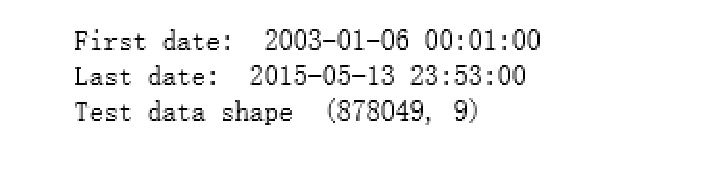
\includegraphics[width=0.9\textwidth]{kaggle/1.eps}
  {\small{Flag.1}}
  \end{minipage}
  \hfill
  \\
  The data ranges from 1/1/2003 to 5/13/2015 creating a training 
  dataset with nine features and 878,049 samples\\
\end{center}
(1) This is meaningless for our analysis and prediction, and it
 needs to be deleted. At the same time, according to the analysis, 
 we can see that there are 67 locations that are wrong in the map. \\
\begin{center}
  \begin{minipage}{0.4\linewidth}
  \centering

  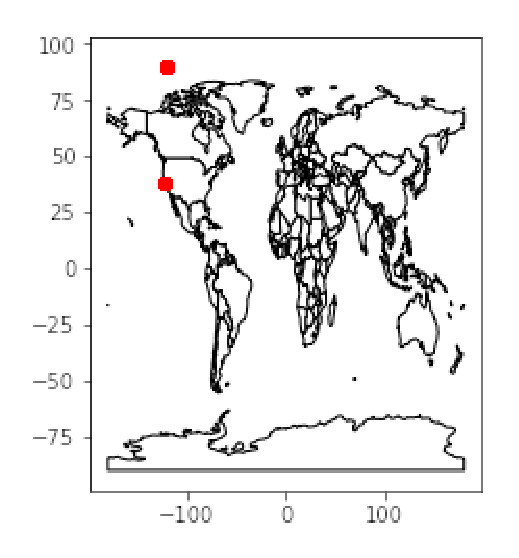
\includegraphics[width=0.9\textwidth]{kaggle/5.eps}
 
  {\small{Flag.2}}

  \end{minipage}
  \hfill
\end{center}
(2)
The following two figures analyze the frequency of criminal incidents in terms of
 days and weeks respectively. It can be seen that there are significant differences 
 between the two figures.
\begin{center}
  \begin{figure}[htbp]
    \centering
    \begin{minipage}[t]{0.48\textwidth}
      \centering
      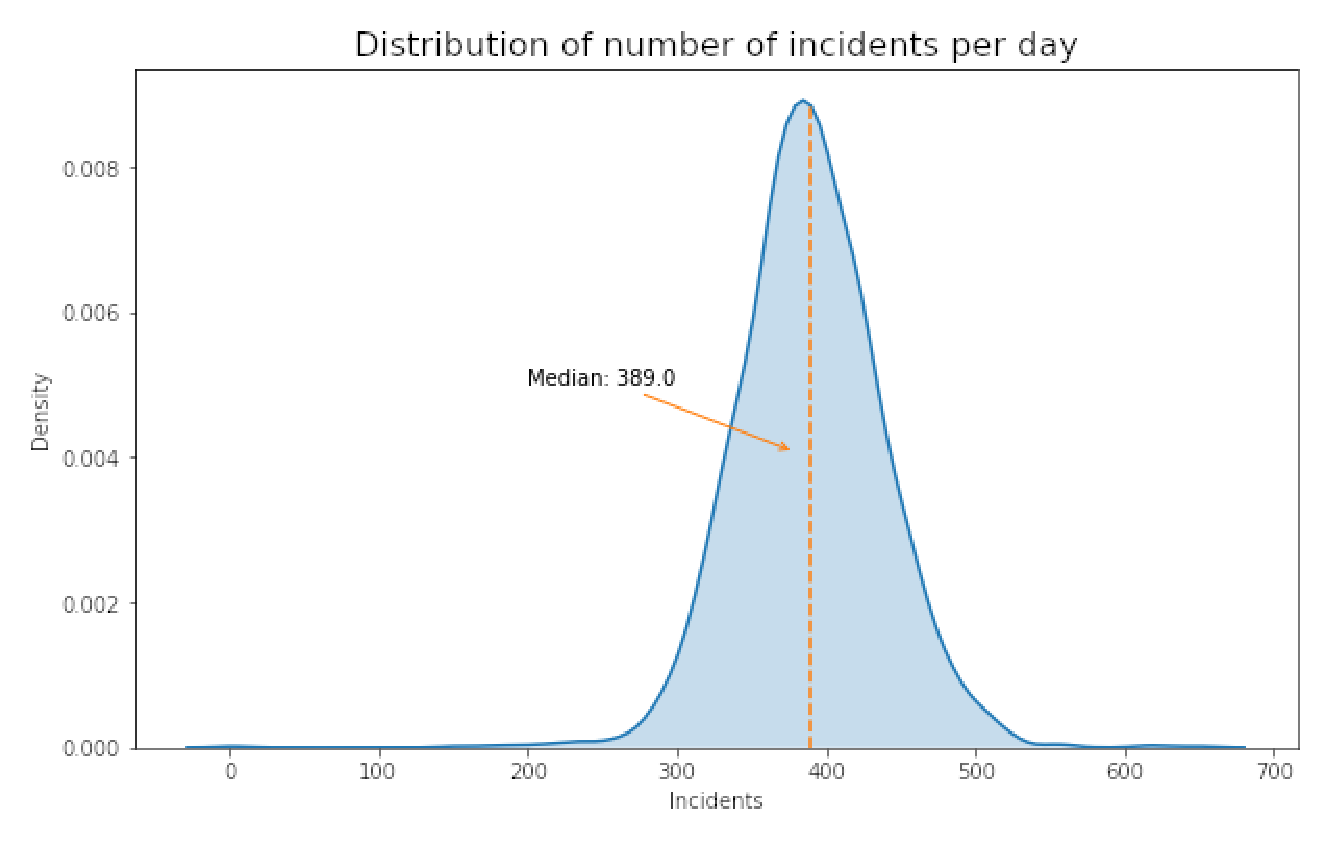
\includegraphics[width=0.9\textwidth]{kaggle/7.1.eps}
      {\small{Flag.3}}
    \end{minipage}
    \begin{minipage}[t]{0.48\textwidth}
      \centering
      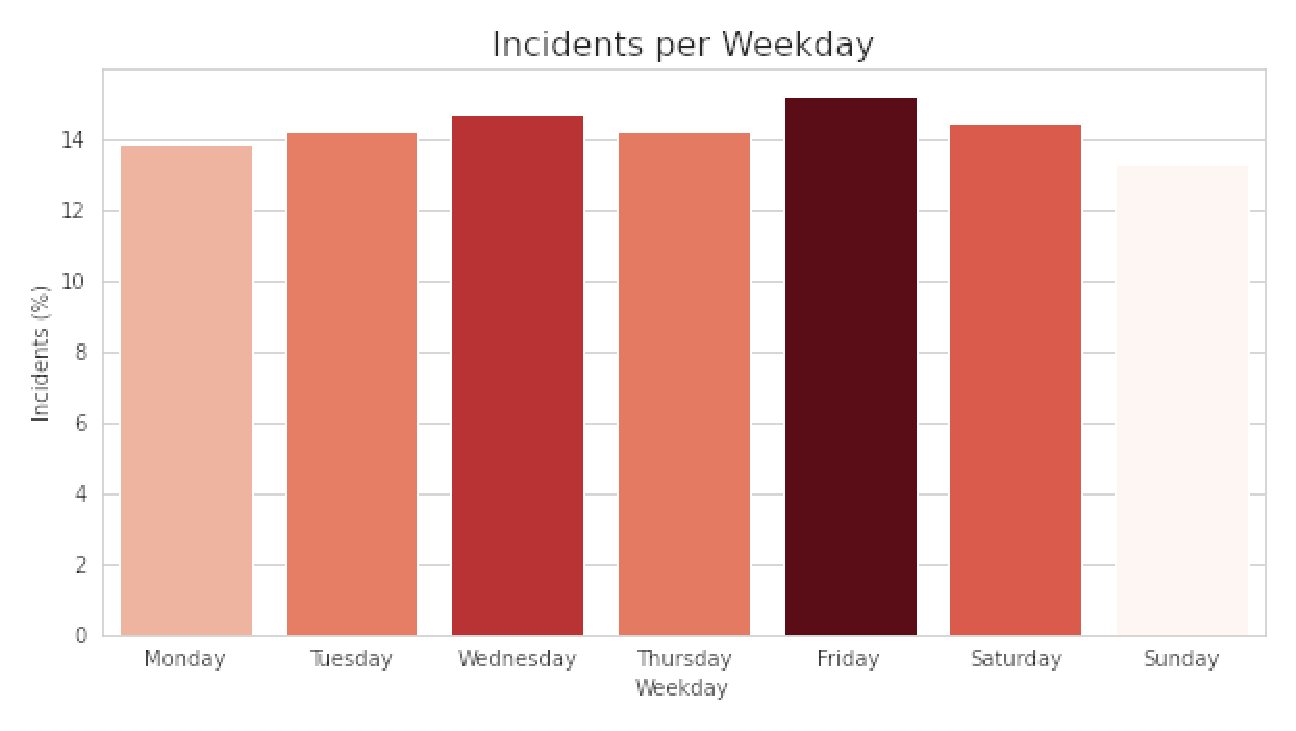
\includegraphics[width=0.9\textwidth]{kaggle/8.1.eps}
      {\small{Flag.4}}
    \end{minipage}
  \end{figure}
  \hfill
  \\
  These variables are distributed uniformly between 1/1/2003 to 5/13/2015
   (and Monday to Sunday) and split between the training and the testing dataset as mentioned before. We did not 
   notice any anomalies on these variables.
   \\
   Also, there is no significant deviation of incidents frequency throughout the week. Thus 
   we do not expect this variable
    to play a significant role in the prediction.
The median frequency of incidents is 389 per day with a standard deviation of 48.51.
\end{center}

(3)There are 39 discrete categories that the police department file the incidents with the 
most common being Larceny/Theft (19.91\%), Non/Criminal (10.50\%),
 and Assault(8.77\%).
\begin{center}
  \begin{minipage}{0.4\linewidth}
  \centering
  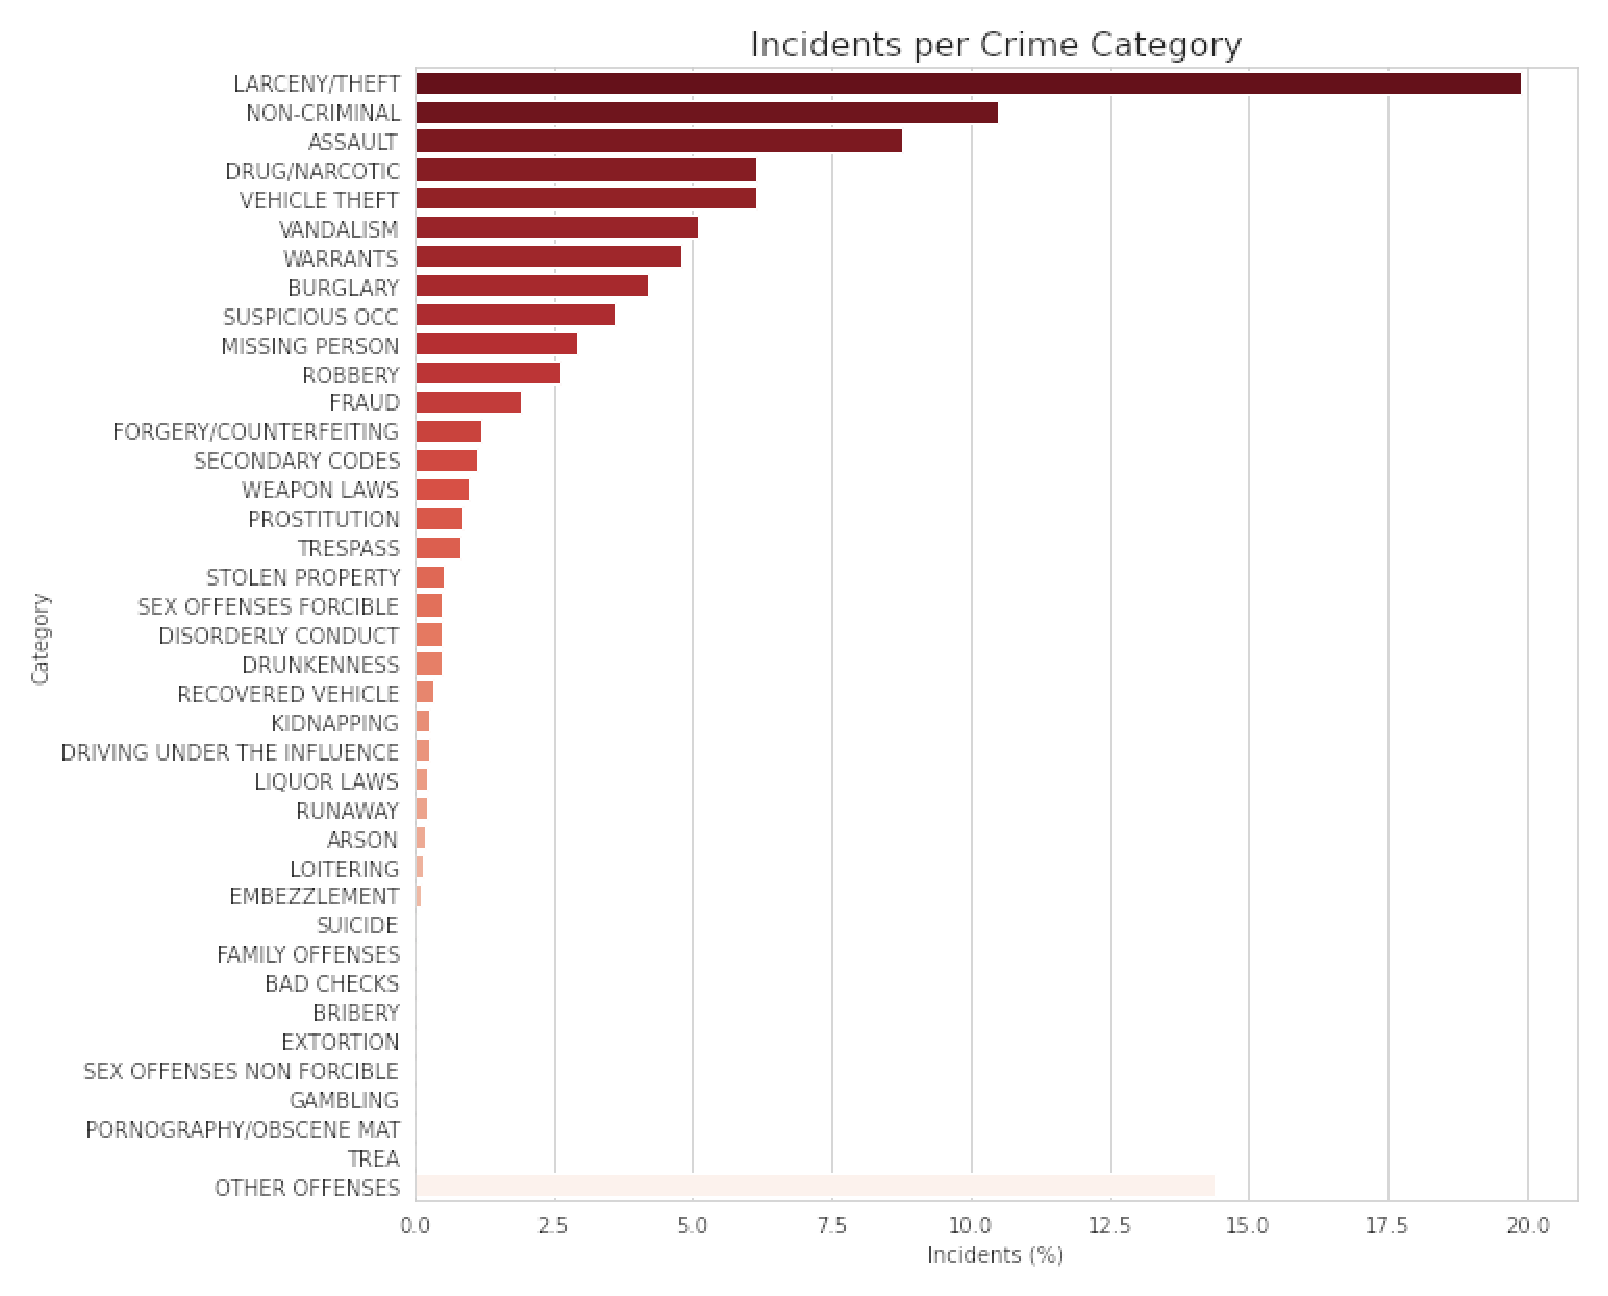
\includegraphics[width=0.9\textwidth]{kaggle/9.eps}
  {\small{Flag.5}}

  \end{minipage}
  \hfill
\end{center}
(4)There are significant differences between the different districts of the City with
the Southern district having the most incidents (17.87\%) followed
by Mission (13.67\%) and Northern (12.00\%).

\begin{center}
  \begin{minipage}{0.4\linewidth}
  \centering

  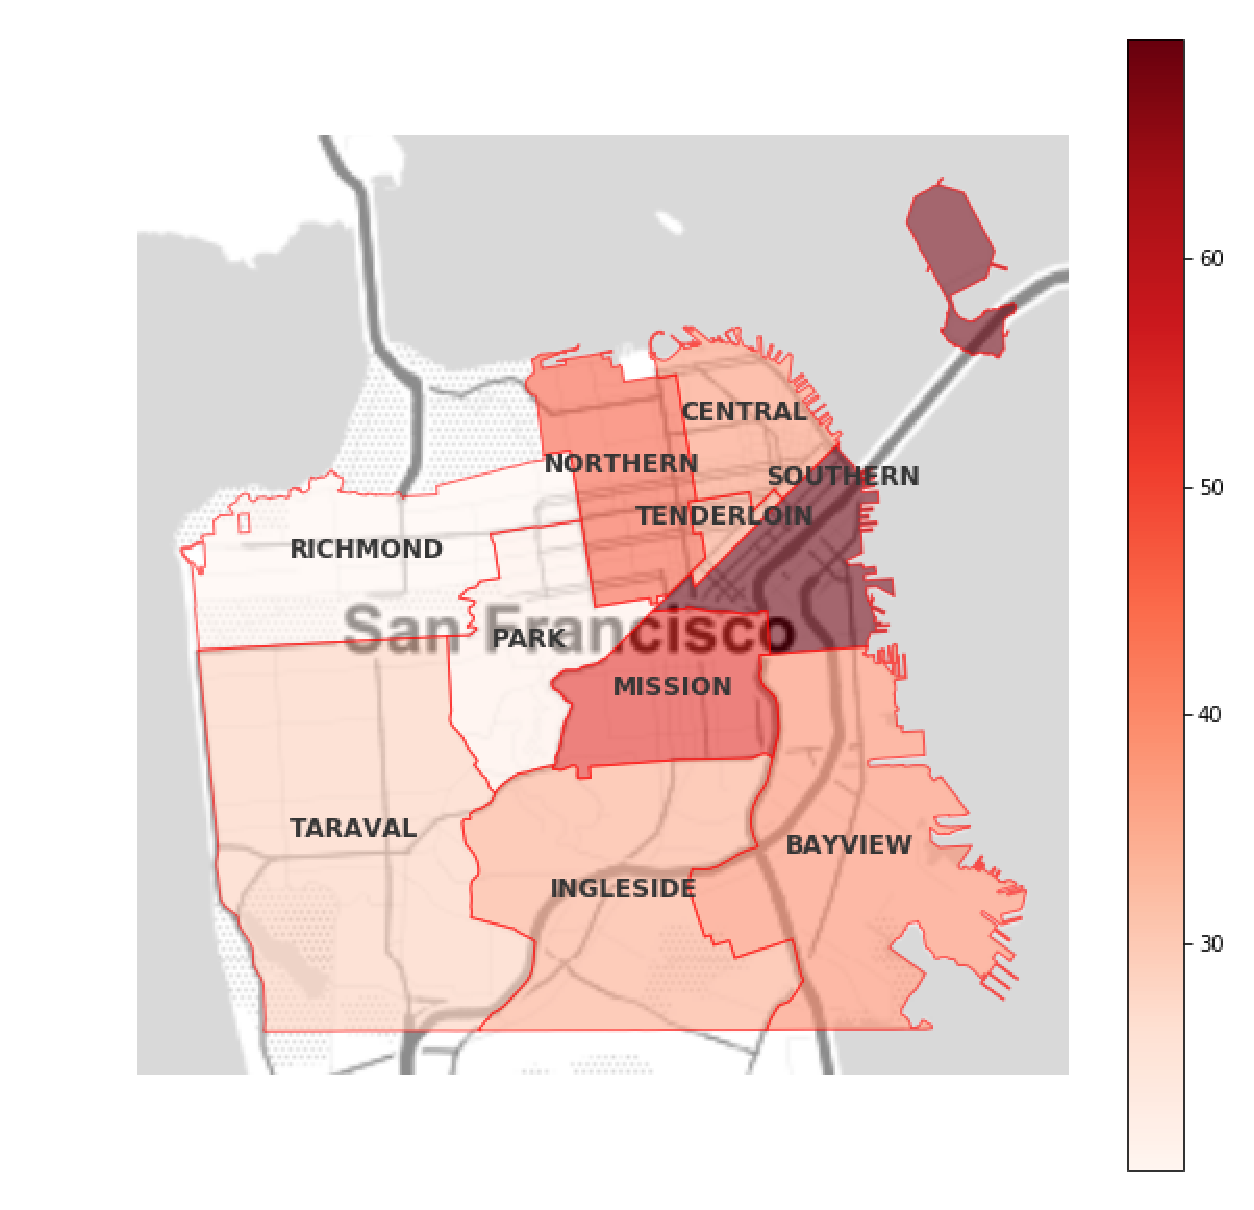
\includegraphics[width=0.9\textwidth]{kaggle/10.eps}
 
  {\small{Flag.5}}

  \end{minipage}
  \hfill
\end{center}
(5)Address
\\
Address, as a text field, requires advanced techniques to use it for
 the prediction. Instead in this project, we will use it to extract
  if the incident has happened on the road or in a building block.
\\
(6)X - Longitude Y - Latitude
We have tested that the coordinates belong inside the boundaries of 
the city. Although longitude does not contain any outliers, latitude 
ludes some 90o values which correspond to the North Pole.
\\

\indent According to the nine features and meanings provided by the data set, we 
analyze them from each Angle and get a different result.Similarly, different 
perspectives will make our analysis
 of data more comprehensive and the results more reliable.

\section{Exploratory Visualization} 


IBased on the Project’s statement, we need to predict the probability of each type of crime
 based on time and location. 
That being said, we present two diagrams to visualize the importance of these variables. 
The first one presents the geographic density of 9 random crime categories. We can see that 
although the epicenter of most of the crimes resides on the northeast of the city, each crime 
has a different density on the rest of the city. This fact is a reliable indication that the
 location ( coordinates / Police District) will be a significant factor for the analysis and
  the forecasting.
\begin{center}

  \begin{minipage}{0.7\linewidth}
  \centering

  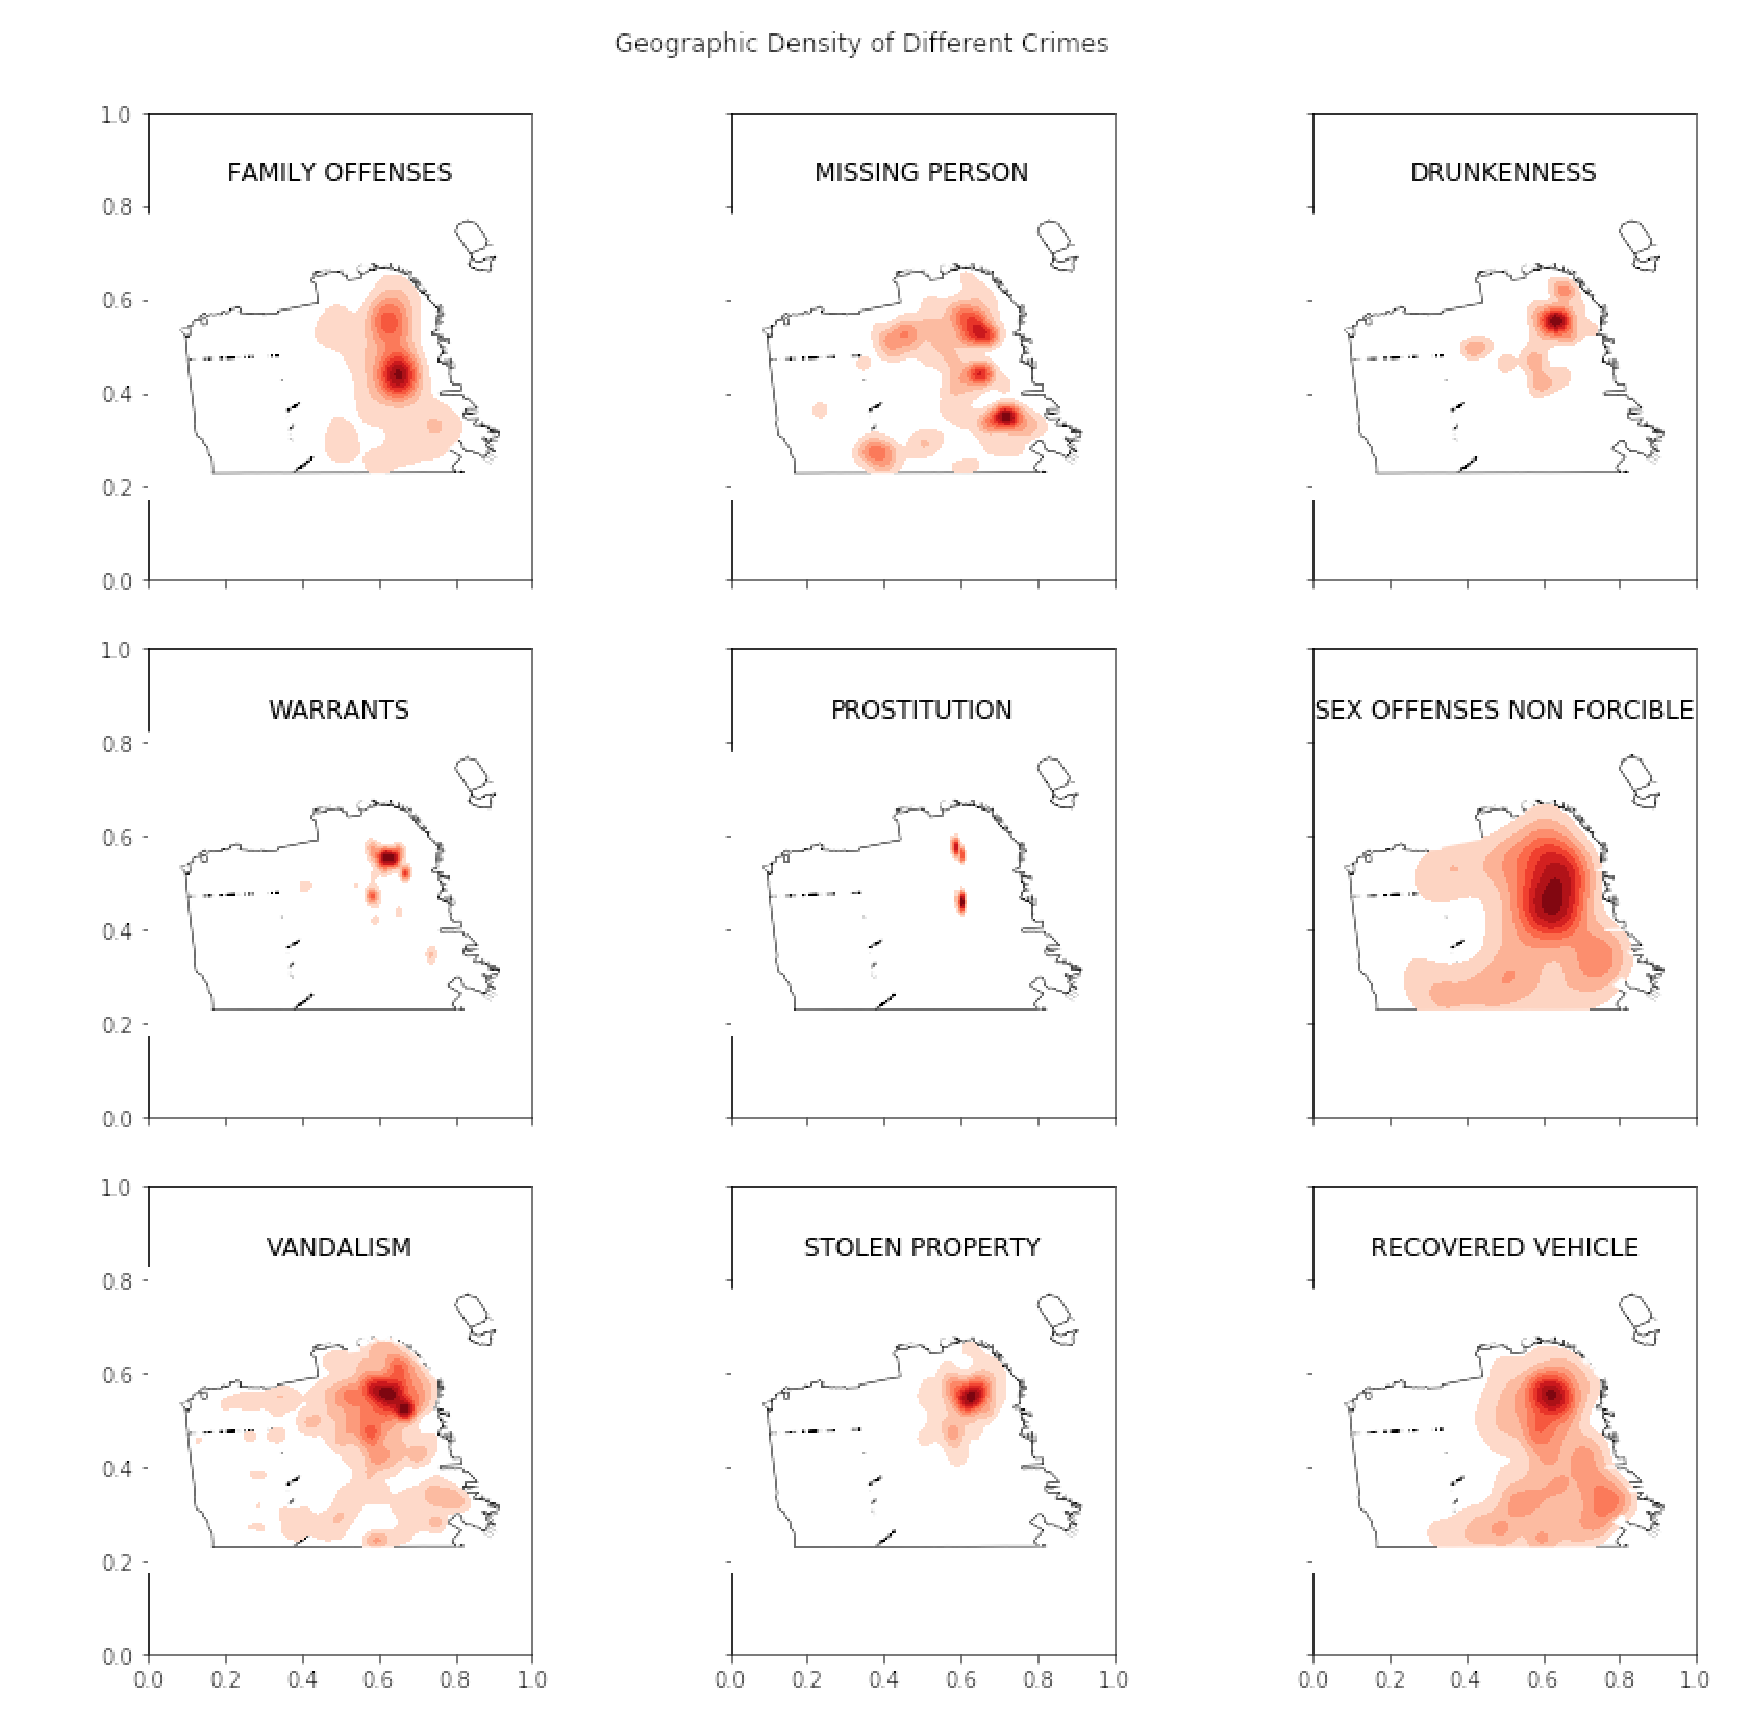
\includegraphics[width=0.9\textwidth]{kaggle/11.1.eps}

  \end{minipage}
\end{center}


The second diagram presents the average number of incidents per hour for five of the crimes' categories.
 It is evident that different crimes have different frequency during
  different times of the day. Some examples are that prostitution 
  picks during the evening and all through the night, Gambling 
  incidents start late at night until the morning and Burglary picks
   early in the morning until the afternoon. As before these are
    sharp pieces of evidence that the time parameters will have a 
    significant role also.
    \begin{center}
      \begin{minipage}{0.7\linewidth}
      \centering
    
      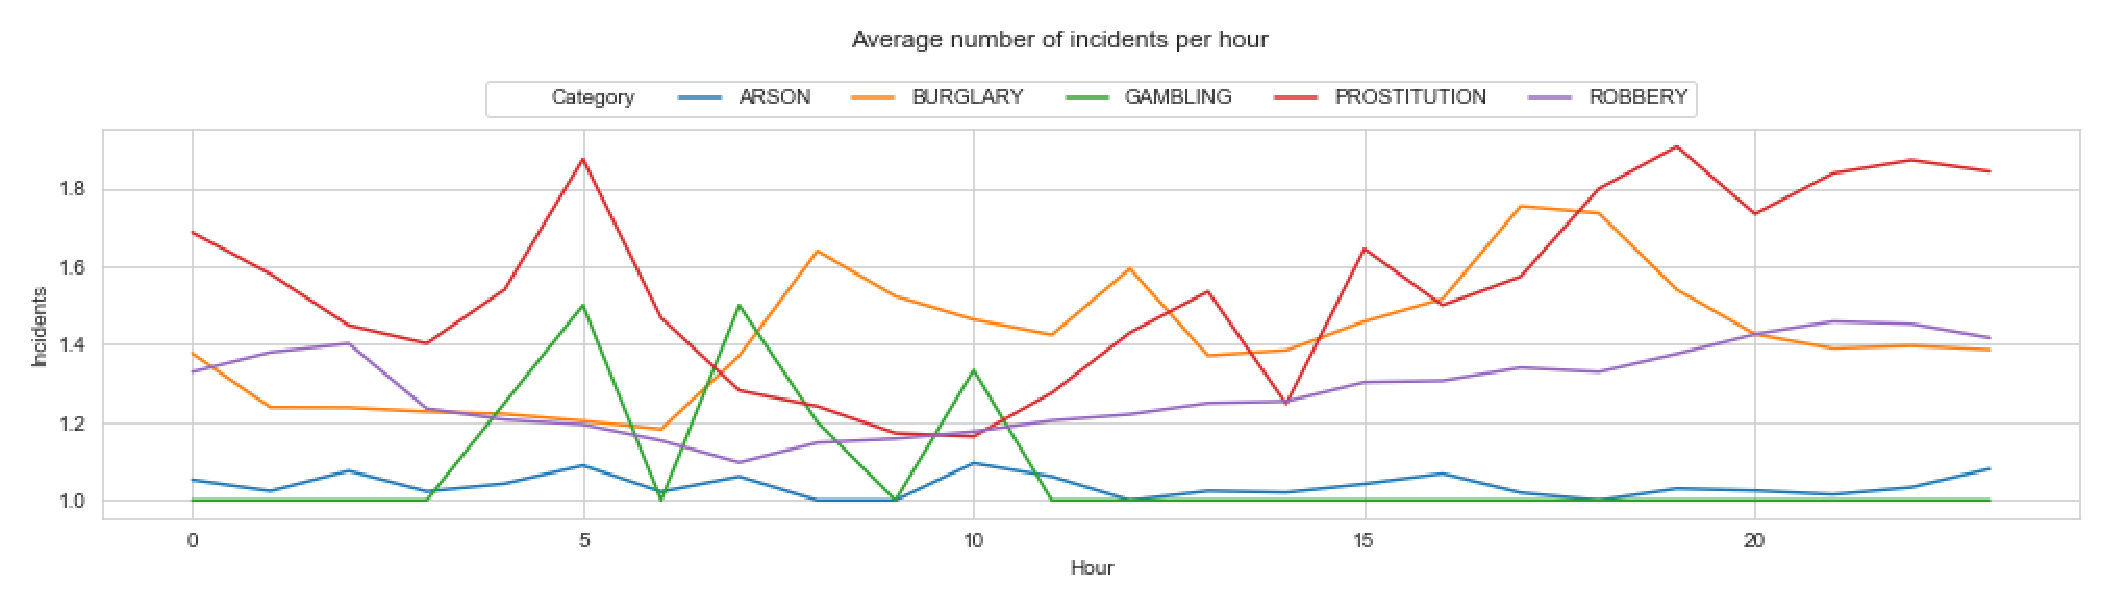
\includegraphics[width=0.9\textwidth]{kaggle/12.eps}
     
      {\small{Flag.5}}
    
      \end{minipage}
      \hfill
    \end{center}
\section{Methodology} \label{sec-experiment}
4.1 Feature Engineering
Then, we created additional features. More specifically:
\begin{itemize}
  \item From the ‘Dates’ field, we extracted the Day, the Month, the Year, the Hour, the Minute, the Weekday, and the number of days since the first day in the data.
  \item From the ‘Address’ field we extracted if the incident has taken place in a crossroad or on a building block.
\end{itemize}


4.2 Feature Selection\\
\indent the feature engineering described above, we ended up with 11 features. 
To identify if any of them increased the complexity of the model without adding 
significant gain to the model, we used the method of Permutation Importance.\\
\\
\indent The idea is that the importance of a feature can be measured by looking 
at how much the loss decreases when a feature is not available. To do that
 we can remove each feature from the dataset, re-train the estimator and 
 check the impact. Doing this would require re-training an estimator for
  each feature, which can be computationally intensive. Instead, we can
replace it with noise by shuffle values for a feature.\\
\\
\indent The implementation of the above technique showed that there is no 
need for any feature removal since all of them have a positive impact 
in the dataset.(1) The update rate of cost function is the cost function
 of mean square error. We can clearly see that after 10 times of 
 updating, the loss value of his cost function remains around 8000.\\
\begin{center}

  \begin{minipage}{0.7\linewidth}
  \centering

  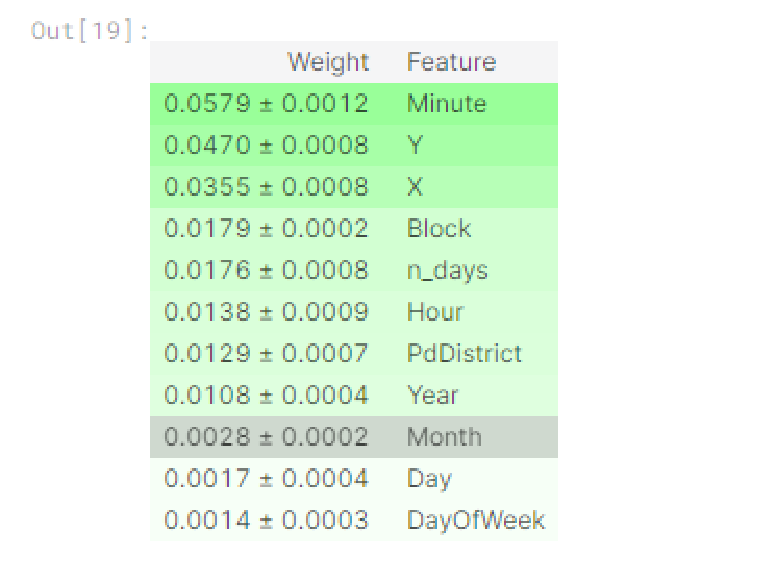
\includegraphics[width=0.9\textwidth]{kaggle/14.eps}
  
  \end{minipage}
\end{center}
\section{Algorithms and Techniques}
The concrete problem is a typical multi-class classification problem, 
and there are several algorithms to solve this problem.First, we evaluated
 several suitable algorithms, from linear models (stochastic gradient descent),
  nearest neighbors (K nearest neighbors), set methods (random forest and AdaBoost), 
  and enhancement algorithms (XGBoost and LIghtGBM), using basic feature engineering and 
default parameters to assess whether they have a clear lead.
\\
\indent LightGBM is a decision tree boosting algorithm uses histogram-based algorithms which bucket continuous feature (attribute) values into discrete bins. This technique speeds up training and reduces memory usage. In layman terms the algorithm works like this:
\\
\indent Fit a decision tree to the data
\\
\indent Evaluate the model
\\
\indent Increase the weight to the incorrect samples.
\\
\indent Choose the leaf with max delta loss to grow.
\\
\indent Grow the tree.
\\
\indent Go to step 2
\section{Conclusions}

This paper mainly abstracts an outline of a crime type and analysis project in San Francisco, and gives the steps required for data processing of a project.Provides a general idea of the shape of a project.At the same time, it also gives some data visualization, which helps us understand the data more intuitively.

% ----------------------------------------------------------------
\newpage
\bibliography{tuliplab,yourbib}
\bibliographystyle{newapa}
%=================================================================

\listoftodos

\end{document}

